\chapter{Resultados e Discussão}

\label{cap:resultados-discussao}

Este capítulo apresenta os resultados do desenvolvimento da plataforma WebGIS ``Sobral em Mapas'', contemplando as ferramentas cartográficas, o gerenciamento administrativo e a integração com serviços WMS e arquivos GeoJSON. Também são examinados o atendimento aos requisitos, as limitações identificadas e a avaliação com usuários ainda em andamento.

\section{Apresentação Geral da Plataforma}

\label{sec:apresentacao-geral-plataforma}

O ``Sobral em Mapas'' consiste em uma plataforma WebGIS destinada à consulta, organização e visualização de informações geoespaciais do município de Sobral, no Ceará. Para atender a essa finalidade, a aplicação reúne ferramentas cartográficas e funcionalidades administrativas em um ambiente web, permitindo tanto a exploração de informações territoriais quanto o gerenciamento dos dados cadastrados. A Figura~\ref{fig:interface-principal} apresenta sua interface principal.

\begin{figure}[!htbp]

    \centering

    \caption{Interface principal da plataforma Sobral em Mapas}

    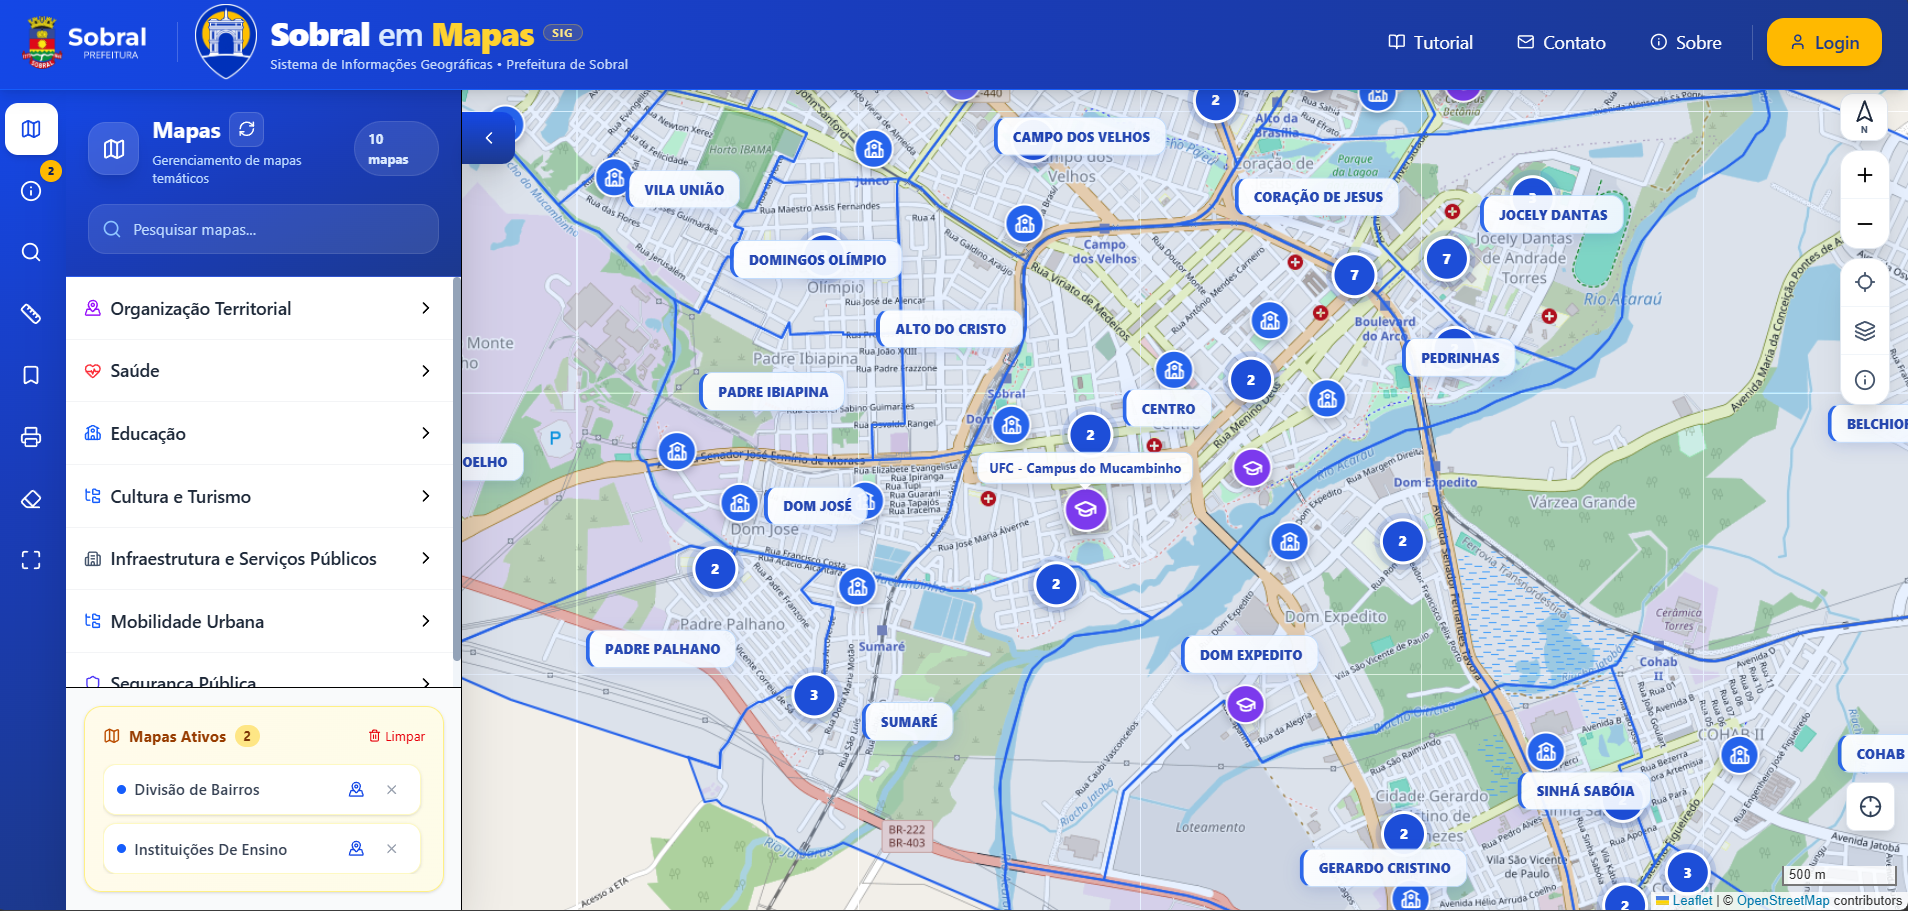
\includegraphics[width=\textwidth]{figuras/interface-principal.png}

    \label{fig:interface-principal}

    \fonte{Elaborado pelo autor.}

\end{figure}

A interface organiza o mapa como elemento central, acompanhado por um cabeçalho, um painel lateral e ferramentas de interação. Na Figura~\ref{fig:interface-principal}, as camadas de bairros e instituições de ensino aparecem simultaneamente, combinando polígonos e marcadores geográficos. A visualização utiliza React e Leaflet, integrados à API Laravel, com suporte a WMS e GeoJSON.

O painel lateral reúne a seleção de camadas, as legendas, a busca de locais, as medições, os favoritos e a impressão. Já os controles sobre o mapa permitem ajustar o zoom, consultar a localização e alternar o mapa-base. Dessa forma, as ferramentas permanecem disponíveis sem interromper a exploração do território.

Para orientar a exploração dos recursos, a plataforma disponibiliza um tutorial interativo acessível pelo cabeçalho, que apresenta as principais ferramentas em etapas e destaca o componente correspondente a cada explicação. Ademais, a página ``Sobre'' reúne informações sobre a proposta do sistema e suas possibilidades de utilização. Esses mecanismos de orientação são acompanhados por ajustes responsivos, de modo que os recursos essenciais permaneçam acessíveis tanto em computadores quanto em dispositivos móveis.

\section{Organização e Visualização das Camadas Temáticas}

\label{sec:visualizacao-camadas}

As informações geoespaciais são agrupadas em categorias e subcategorias, facilitando a localização das camadas. Essa organização é carregada dinamicamente da API Laravel e pode ser atualizada no ambiente administrativo sem exigir alterações no código da interface.

A Figura~\ref{fig:organizacao-camadas} exemplifica essa organização por meio da categoria Educação, da subcategoria Instituições de Ensino e da respectiva camada ativada. No mapa, os estabelecimentos educacionais aparecem como marcadores e rótulos, enquanto o painel de mapas ativos permite acompanhar e remover as camadas selecionadas. Desse modo, a imagem evidencia a integração entre a navegação temática e a visualização cartográfica.

As categorias e subcategorias podem ser expandidas ou recolhidas para reduzir o excesso de informações. Como as camadas são ativadas individualmente, é possível combinar temas e remover os mapas selecionados. Além disso, a ferramenta de enquadramento permite visualizar a extensão geográfica das camadas GeoJSON.

Para facilitar consultas recorrentes, o usuário também pode marcar camadas como favoritas. Já no painel de informações, cada camada ativa apresenta uma legenda associada à sua representação cartográfica. No caso dos arquivos GeoJSON, a simbologia considera o tipo de geometria e as propriedades visuais disponíveis, permitindo ajustes temporários de cor e de exibição dos nomes sem modificar os arquivos originais. Com isso, torna-se mais simples distinguir camadas sobrepostas e adaptar a apresentação dos dados às necessidades de leitura.

\begin{figure}[!htbp]

    \centering

    \caption{Organização temática e seleção de camadas na plataforma Sobral em Mapas}

    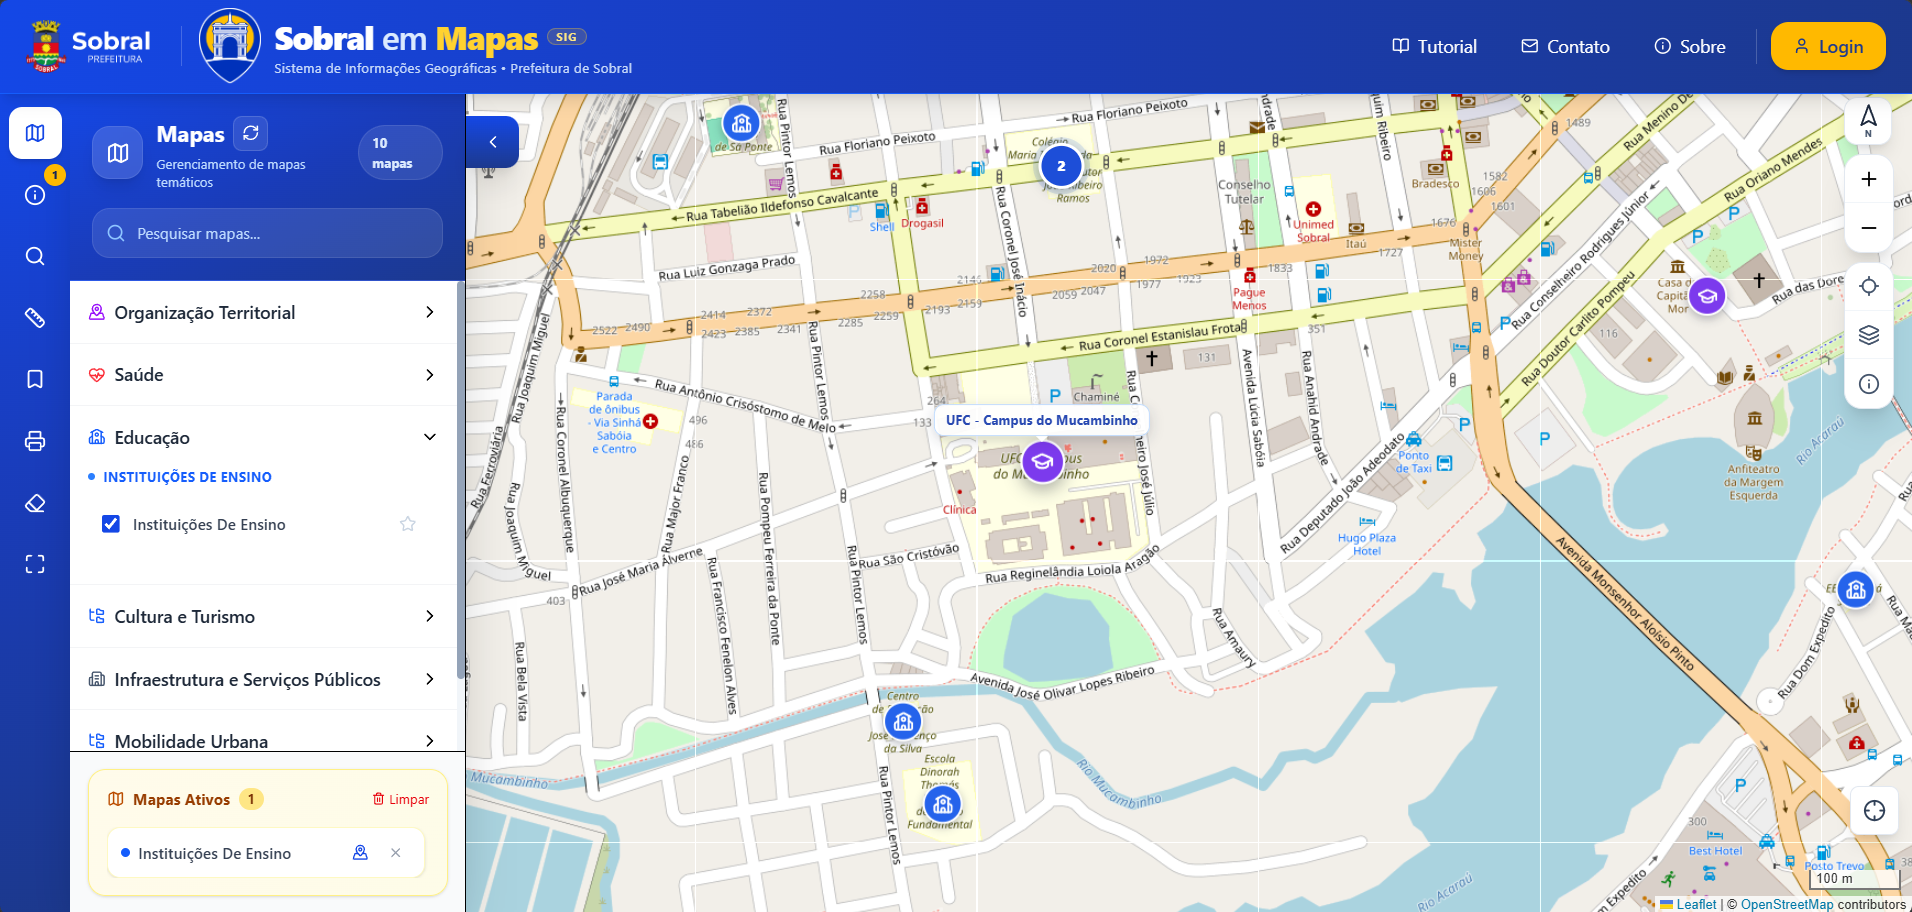
\includegraphics[width=\textwidth]{figuras/organizacao-camadas.png}

    \label{fig:organizacao-camadas}

    \fonte{Elaborado pelo autor.}

\end{figure}

\section{Representação e Consulta de Dados Geoespaciais}

\label{sec:visualizacao-geoespacial}

A plataforma visualiza camadas provenientes de serviços WMS e arquivos GeoJSON, reunindo informações espaciais de diferentes origens. O uso do GeoJSON permite carregar dados vetoriais no navegador e consultar atributos das feições, ampliando as alternativas de disponibilização das informações cartográficas para os usuários.

A Figura~\ref{fig:visualizacao-geoespacial} apresenta a camada Divisão de Distritos por meio de polígonos e rótulos. No painel do distrito Sede, são exibidos atributos como área, nome e identificador, ilustrando a consulta de informações associadas à geometria selecionada.

A consulta às feições GeoJSON ocorre pela seleção de pontos, linhas ou polígonos no mapa. A aplicação apresenta uma janela de informações (\textit{popup}) com título e atributos da feição. Para facilitar a leitura, os campos recebem rótulos claros e as medidas de área e comprimento aparecem em unidades adequadas, sem alterar os valores originais armazenados.

A representação dos pontos utiliza símbolos temáticos definidos pelos atributos das feições, permitindo diferenciar instituições de ensino, serviços de saúde e outros locais. A exibição de ícones e rótulos também varia conforme o nível de zoom, evitando o excesso de elementos em escalas mais afastadas e melhorando a legibilidade.

\begin{figure}[!htbp]

    \centering

    \caption{Visualização da divisão distrital e consulta de atributos geográficos}

    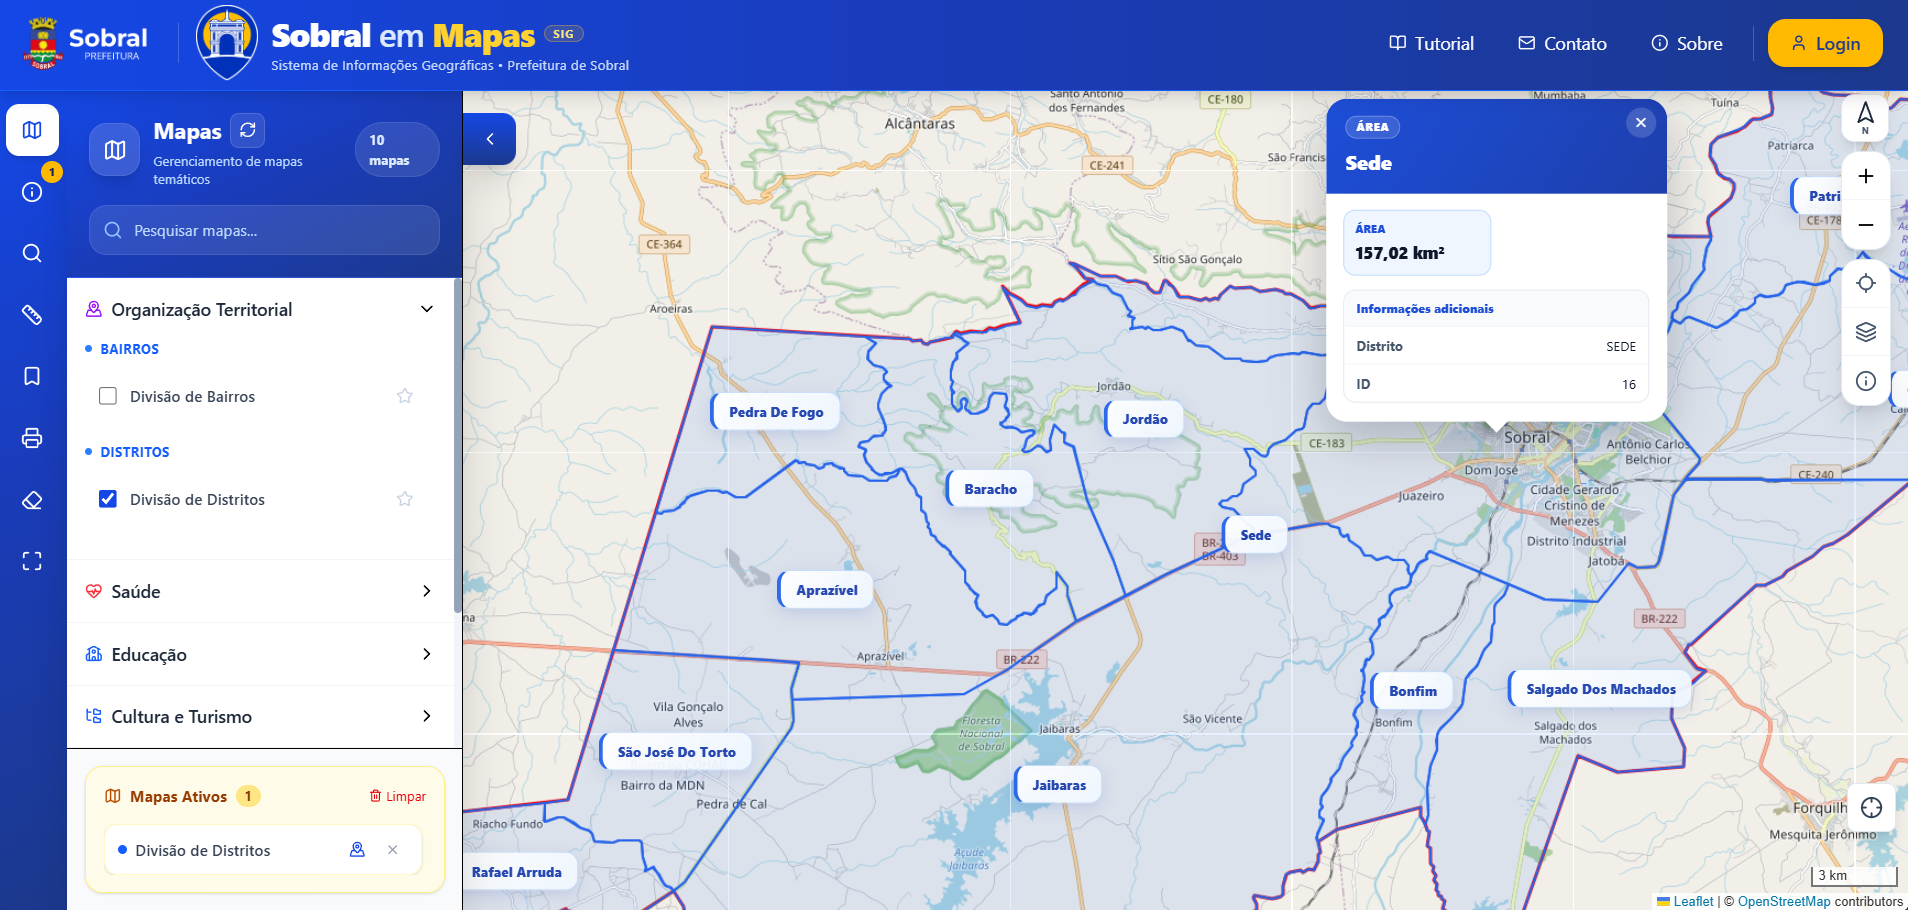
\includegraphics[width=\textwidth]{figuras/visualizacao-geoespacial.png}

    \label{fig:visualizacao-geoespacial}

    \fonte{Elaborado pelo autor.}

\end{figure}

\FloatBarrier

\section{Ferramentas de Interação Cartográfica}

\label{sec:ferramentas-cartograficas}

A plataforma também oferece busca de localizações, medições, favoritos, limpeza do mapa, tela cheia e impressão. Essas ferramentas ampliam a exploração do território e permitem executar operações cartográficas na própria interface, sem recorrer a outros programas.

Na ferramenta de busca, o usuário pode pesquisar endereços, pontos de interesse e coordenadas. O campo sugere locais das camadas GeoJSON e mantém um histórico recente no navegador. Nas consultas externas, um serviço de geocodificação localiza o resultado e centraliza o mapa, exibindo um marcador com informações correspondentes.

As ferramentas de medição permitem desenhar linhas e áreas para obter, respectivamente, distâncias e medidas de superfície. Os resultados são reunidos em um painel no qual os elementos podem ser consultados e excluídos individualmente. Além disso, o usuário pode escolher unidades em metros ou quilômetros para distâncias e em metros quadrados ou quilômetros quadrados para áreas, bem como ajustar cor, espessura e opacidade dos desenhos para diferenciá-los das demais informações cartográficas.

A Figura~\ref{fig:medicao-impressao} apresenta medições e exportação, com uma área de 52.223,15 m² e uma distância de 232,01 m exibidas no painel lateral. Também mostra a seleção de uma região para exportação em PDF, PNG ou JPEG, permitindo compartilhar a visualização do mapa.

Para exportar o mapa, o usuário delimita uma região da visualização por meio de uma área de seleção ajustável e escolhe o formato desejado. A plataforma também permite alternar entre mapas-base, incluindo representações de ruas, imagens de satélite e visualização topográfica, conforme a disponibilidade das fontes configuradas. Dessa maneira, os recursos de exportação se somam aos controles de zoom, localização e tela cheia, oferecendo diferentes formas de explorar o território sem alterar as camadas cadastradas.

\begin{figure}[H]

    \centering

    \caption{Ferramentas de medição e impressão cartográfica da plataforma}

    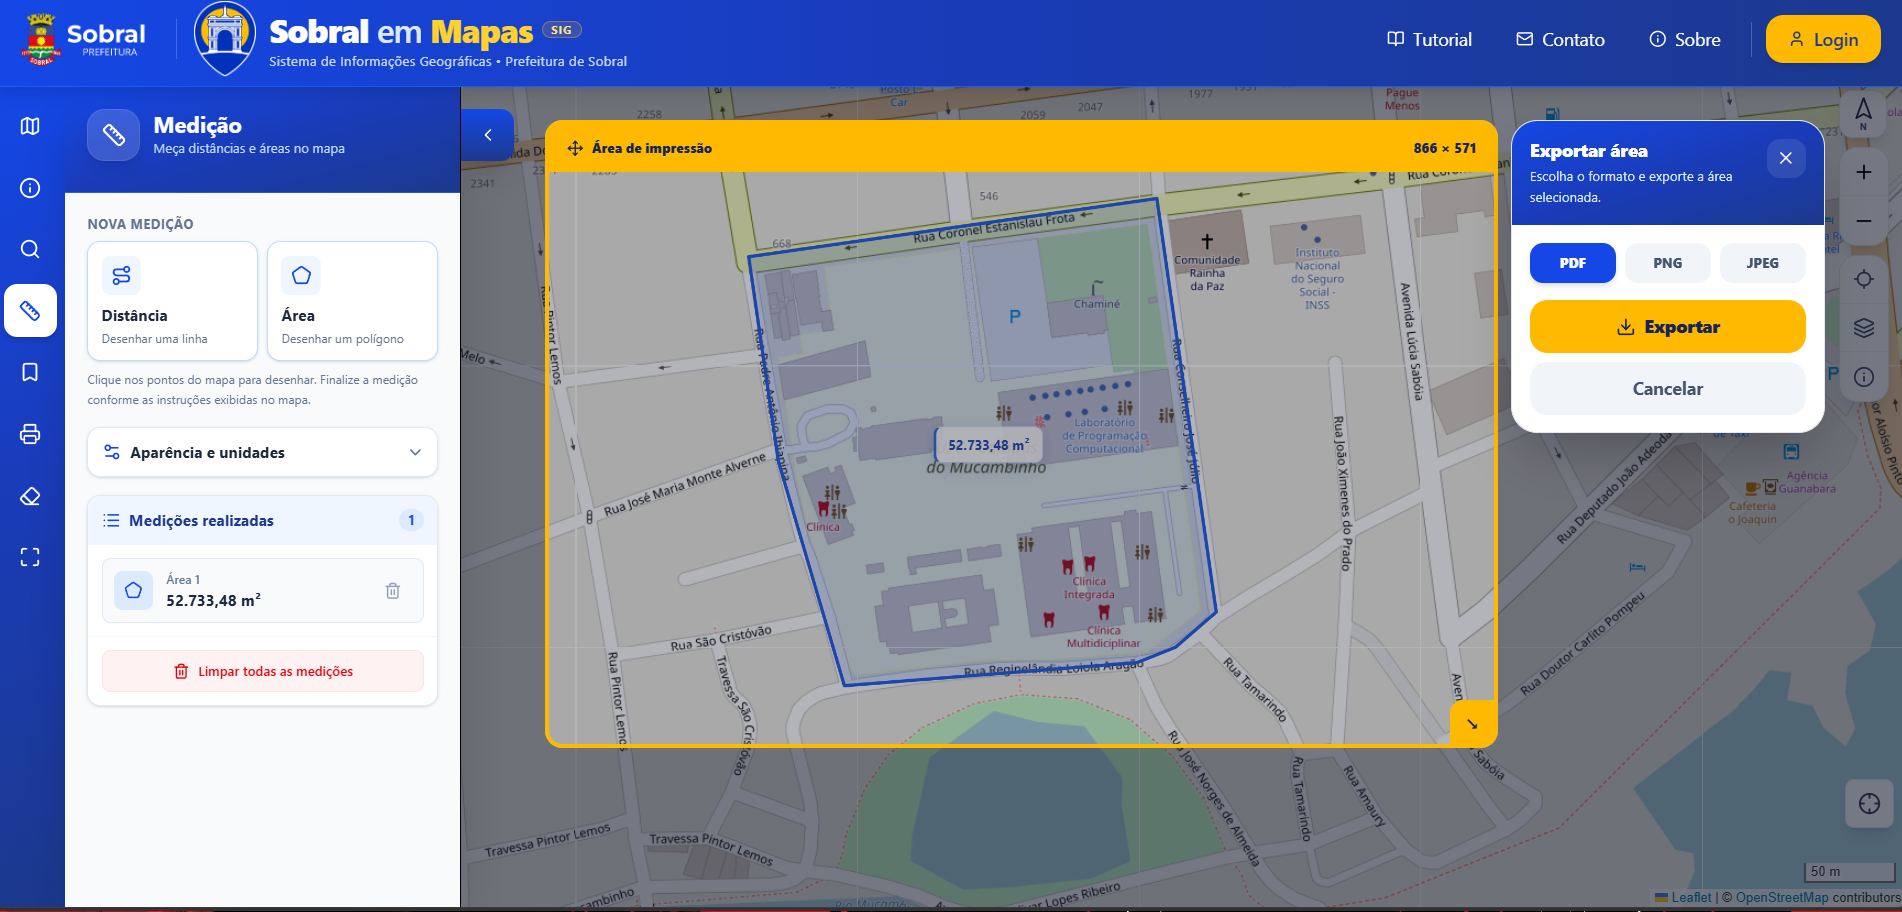
\includegraphics[width=\textwidth]{figuras/medicao-impressao.png}

    \label{fig:medicao-impressao}

    \fonte{Elaborado pelo autor.}

\end{figure}

\section{Ambiente Administrativo da Plataforma}

\label{sec:ambiente-administrativo}

A plataforma dispõe de um ambiente administrativo para gerenciar informações exibidas no mapa. Seu acesso é restrito a usuários autenticados e autorizados, pois reúne operações sobre categorias, subcategorias, camadas, serviços WMS e contas cadastradas. Dessa forma, as funções administrativas permanecem separadas das consultas públicas.

A área administrativa está organizada em páginas de gerenciamento. Enquanto categorias e subcategorias mantêm a organização temática do mapa, as páginas de usuários e solicitações de cadastro permitem acompanhar perfis de acesso e pedidos de aprovação. As operações disponíveis em cada página dependem das permissões do usuário autenticado.

Entre os recursos implementados, destaca-se o gerenciamento de camadas, que permite cadastrar, consultar, editar, ativar, desativar e excluir registros geográficos. A Figura~\ref{fig:gerenciamento-camadas} apresenta a interface correspondente, com indicadores sobre a quantidade de camadas, sua situação de ativação e a visibilidade pública. Além desses indicadores, a página reúne uma tabela com os registros e ferramentas de busca e administração, contemplando tanto camadas associadas a serviços WMS quanto arquivos GeoJSON.

A listagem também apresenta a origem dos dados, sua classificação temática e as condições de publicação de cada camada. Nesse ambiente, a pesquisa textual e os filtros por situação facilitam a localização dos registros, enquanto ações específicas permitem alterar o estado de uma camada, editar seus metadados, excluir o cadastro ou obter o arquivo geográfico, quando disponível. Dessa forma, as operações ficam concentradas em uma interface, e as alterações administrativas podem ser refletidas posteriormente na consulta cartográfica pública.

\begin{figure}[H]

    \centering

    \caption{Interface administrativa de gerenciamento de camadas geográficas}

    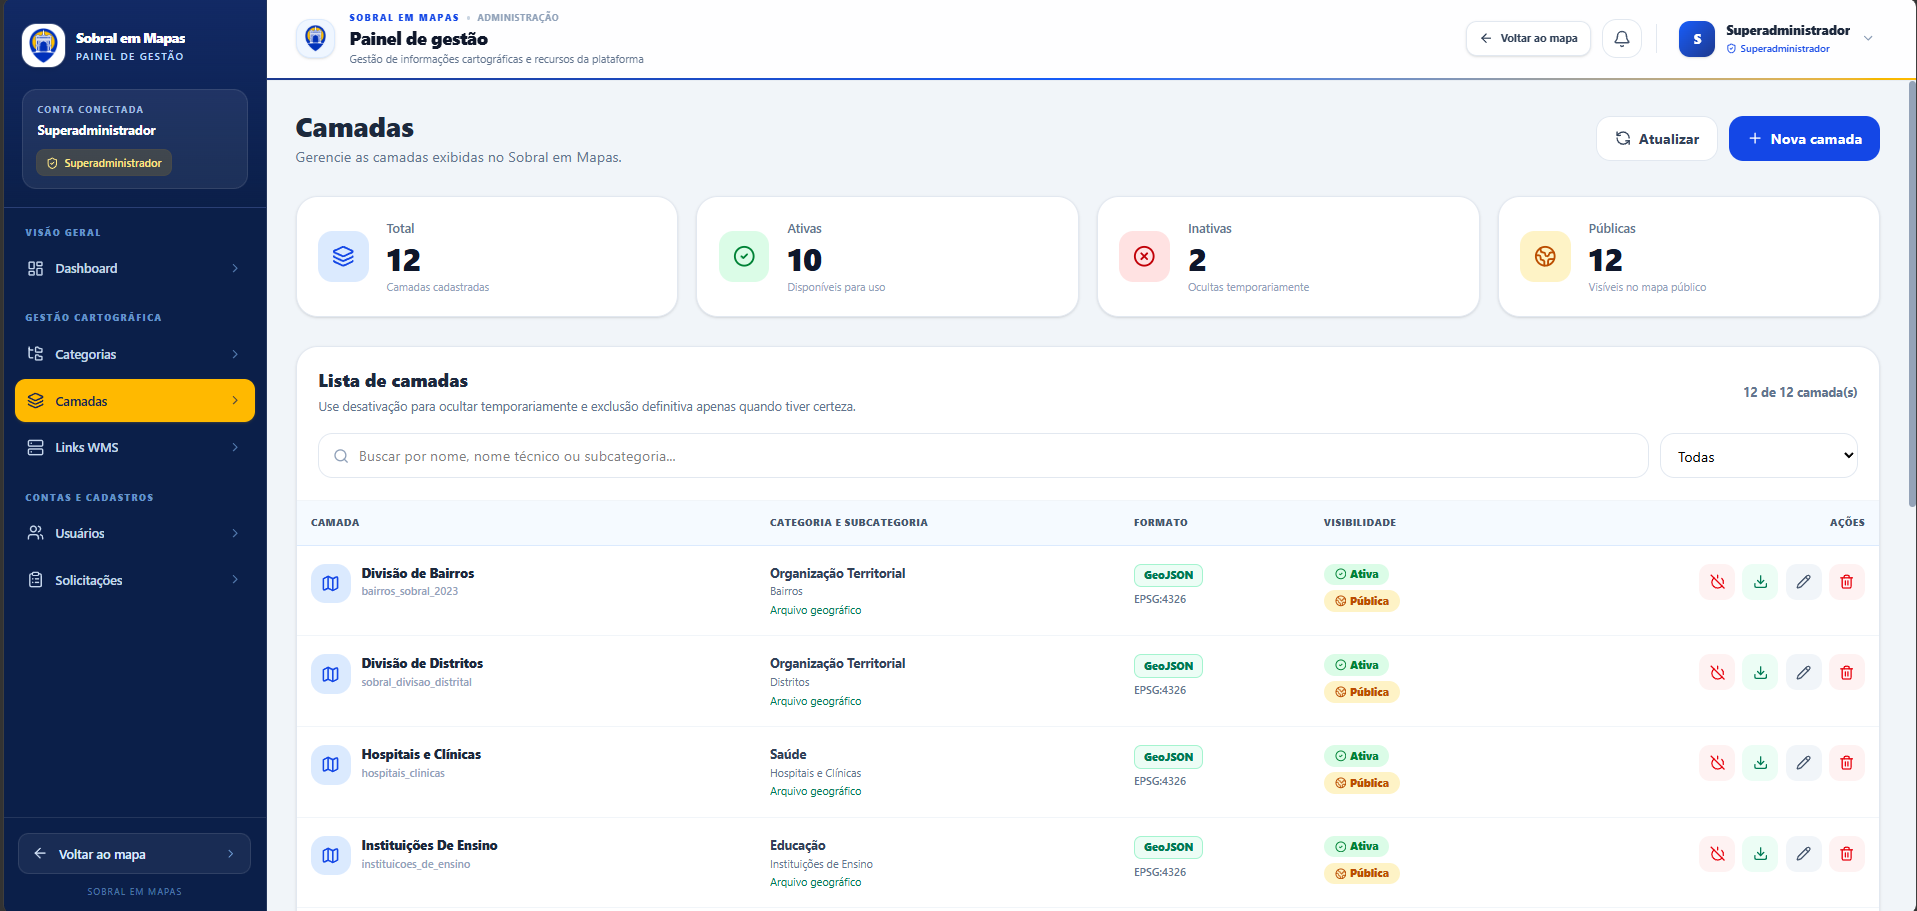
\includegraphics[width=\textwidth]{figuras/gerenciamento-camadas.png}

    \label{fig:gerenciamento-camadas}

    \fonte{Elaborado pelo autor.}

\end{figure}

O cadastro de camadas permite selecionar a fonte cartográfica e informar os metadados necessários à sua organização. Para os arquivos GeoJSON, o formulário oferece a seleção de conteúdos já armazenados ou o envio de novos dados, ambos acompanhados de uma pré-visualização cartográfica. A Figura~\ref{fig:cadastro-geojson} apresenta esse processo com um arquivo de instituições de ensino, permitindo observar sua distribuição espacial antes da conclusão do cadastro.

Para facilitar o cadastro, o formulário organiza em etapas a identificação, a seleção do arquivo e as configurações de apresentação e publicação. Os campos obrigatórios exibem mensagens de validação quando faltam nome, classificação temática ou arquivo geográfico. A biblioteca permite reutilizar arquivos GeoJSON e a pré-visualização mostra seu conteúdo, embora o envio de novas camadas esteja atualmente concentrado nesse formato.

\begin{figure}[H]

    \centering

    \caption{Cadastro de camada GeoJSON com pré-visualização cartográfica}

    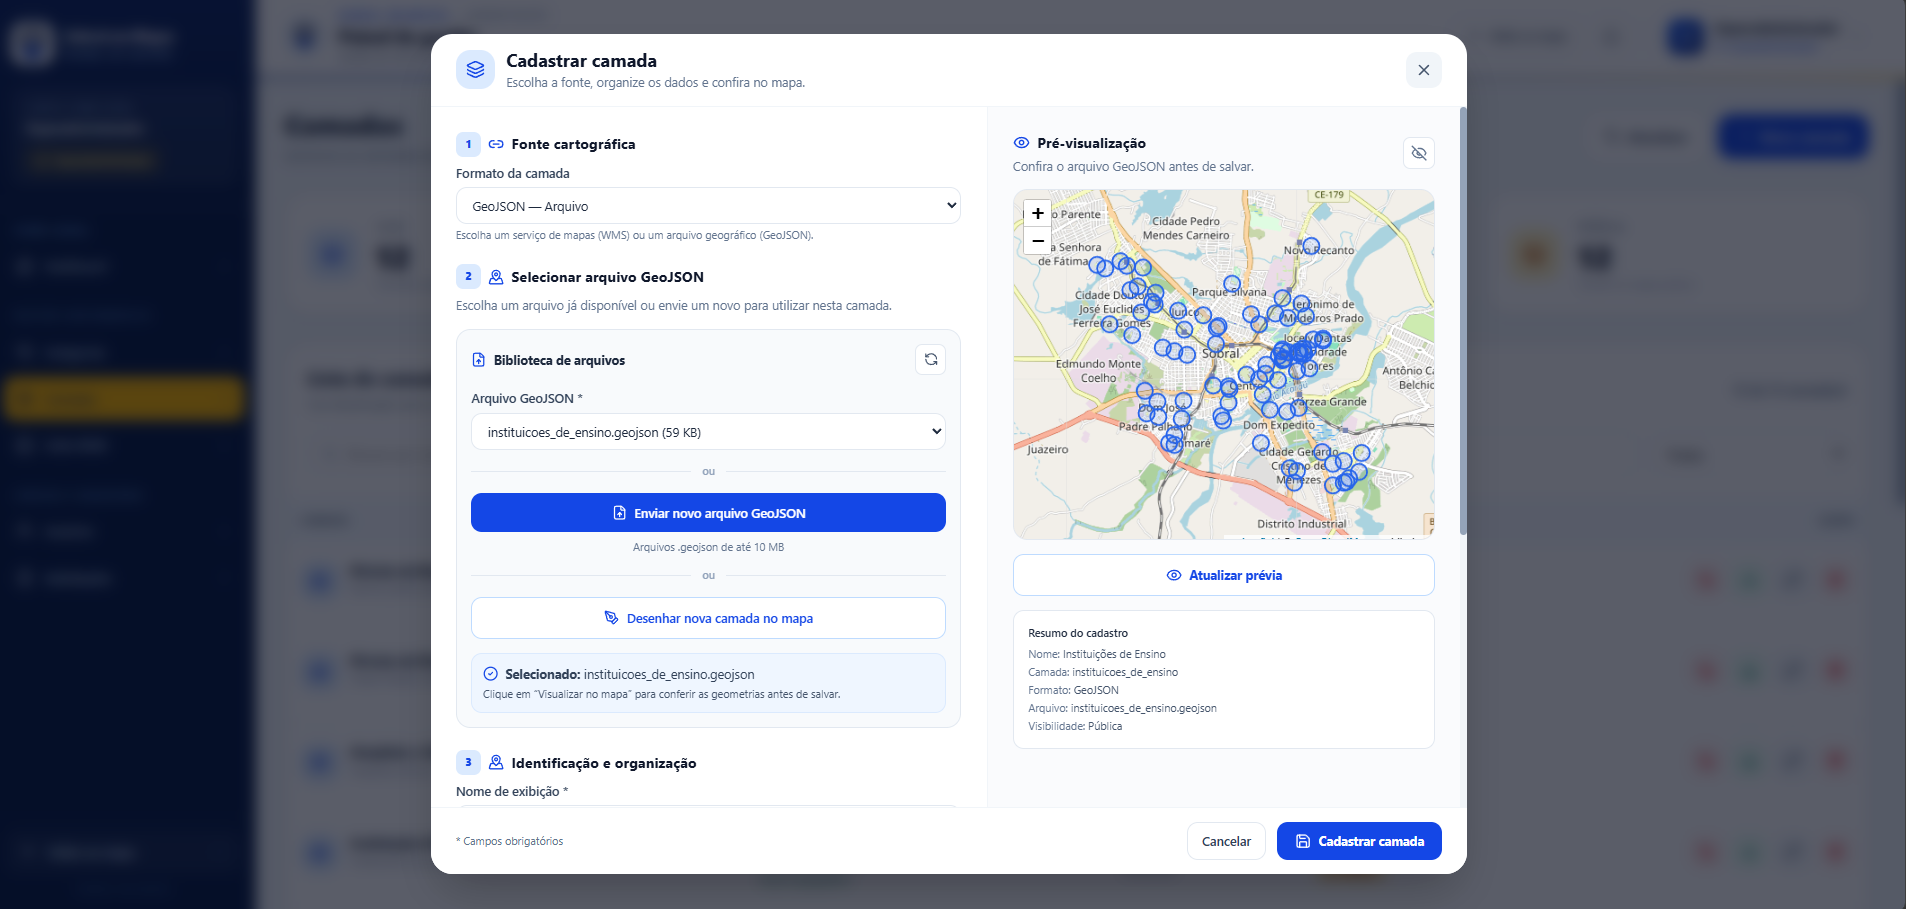
\includegraphics[width=\textwidth]{figuras/cadastro-geojson.png}

    \label{fig:cadastro-geojson}

    \fonte{Elaborado pelo autor.}

\end{figure}

Além do envio de arquivos, foi implementado um editor GeoJSON integrado ao ambiente administrativo, que permite criar e modificar feições no mapa. A ferramenta oferece desenho de pontos, linhas e polígonos, edição de geometrias e ajustes de cor e espessura. A Figura~\ref{fig:editor-geojson} apresenta o editor com instituições de ensino carregadas e seus controles disponíveis.

O editor também oferece opções para desenhar retângulos e círculos, além de editar, excluir, desfazer e refazer operações. Durante a criação das feições, podem ser ajustados cores, estilos de linha, preenchimentos e tamanhos dos pontos, bem como consultadas as medidas das geometrias. Os atributos podem ser alterados antes do salvamento e o conteúdo resultante é convertido para GeoJSON. No caso dos círculos, utiliza-se uma aproximação poligonal, visto que o formato não possui um tipo geométrico específico para representá-los.

\begin{figure}[H]

    \centering

    \caption{Editor de geometrias GeoJSON integrado ao ambiente administrativo}

    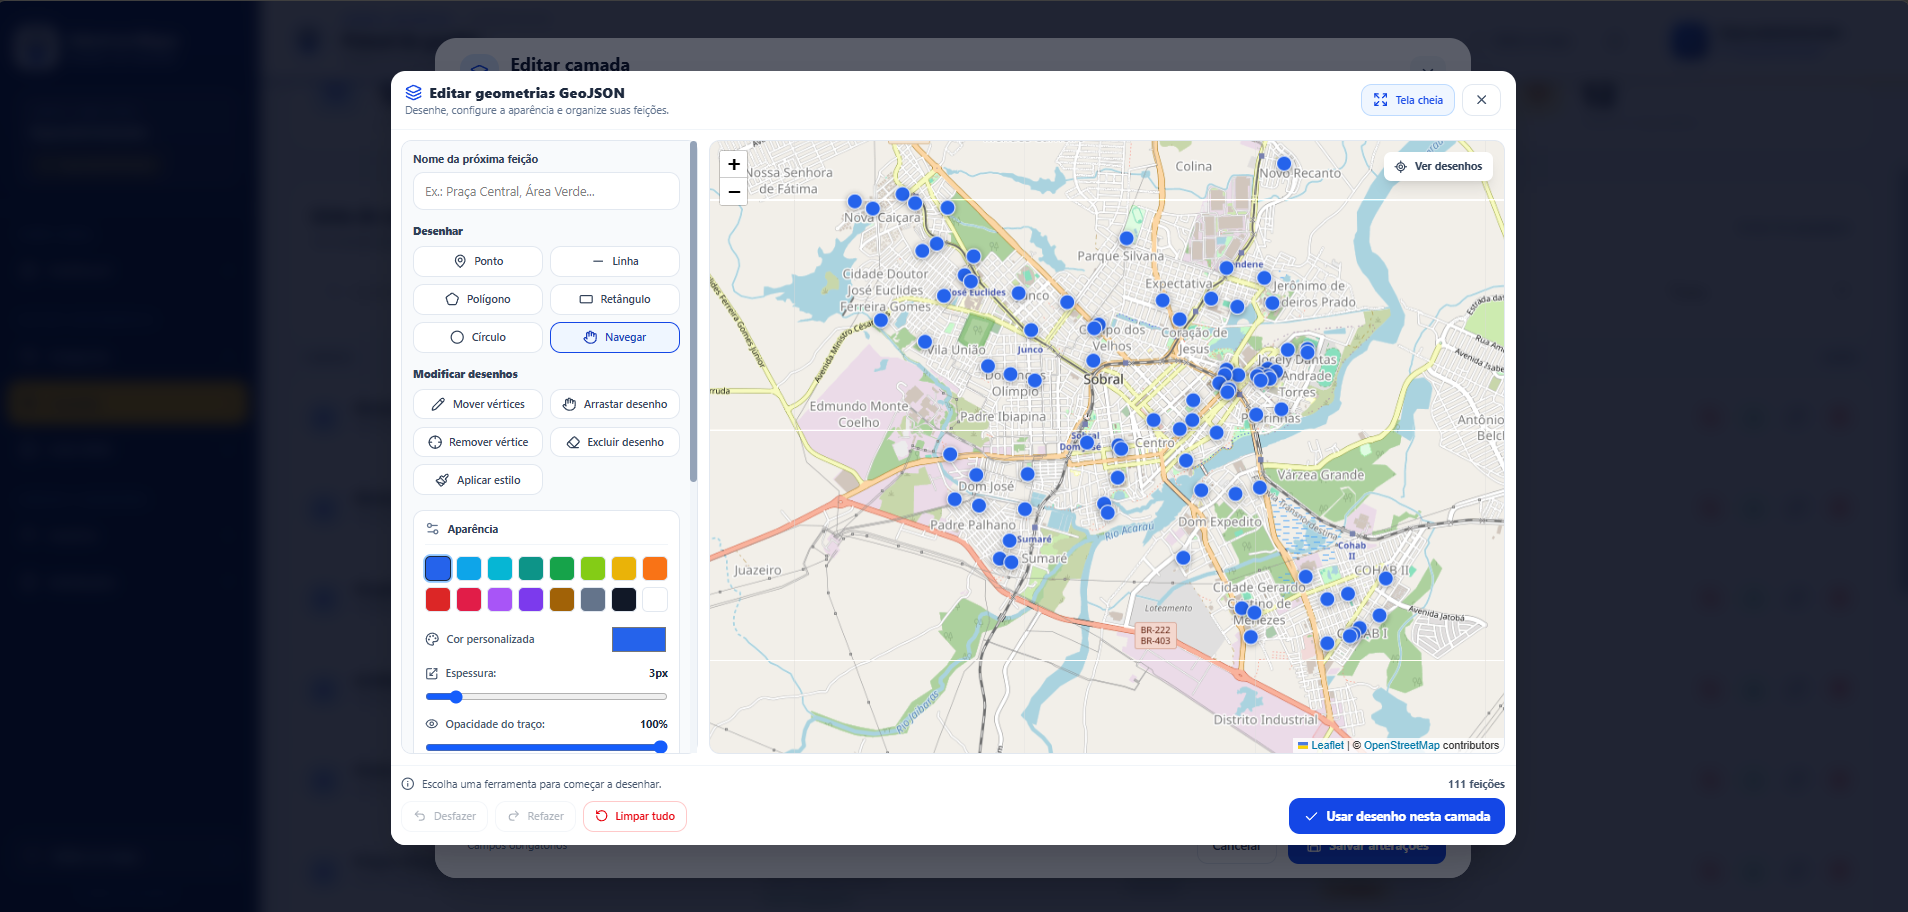
\includegraphics[width=\textwidth]{figuras/editor-geojson.png}

    \label{fig:editor-geojson}

    \fonte{Elaborado pelo autor.}

\end{figure}

Esses recursos ampliam o gerenciamento geográfico por permitir incorporar arquivos vetoriais e editar geometrias na plataforma. Assim, o ambiente administrativo organiza as camadas e disponibiliza suas informações na interface pública.

\section{Implantação e Ambiente de Execução}

\label{sec:implantacao-ambiente-execucao}

Após a integração das funcionalidades, o ``Sobral em Mapas'' foi disponibilizado em nuvem com cliente cartográfico e servidor separados. O \textit{front-end}, desenvolvido em React, foi publicado na Vercel a partir do processo de compilação do Vite. Já o \textit{back-end}, em Laravel, foi implantado no Railway para executar a API. Os componentes se comunicam por endereços definidos em variáveis de ambiente e podem ser atualizados de maneira independente.

Para o desenvolvimento e a execução local, foi utilizado o Docker, que organiza o servidor de aplicação, o banco de dados e os serviços auxiliares em contêineres. Essa configuração contribui para a padronização do ambiente, facilitando as atividades de desenvolvimento e verificação do sistema. A Figura~\ref{fig:implantacao-ambientes} apresenta os três ambientes utilizados, reunindo a publicação da interface na Vercel, a execução da API no Railway e a organização dos contêineres no Docker.

\begin{figure}[H]

    \centering

    \caption{Ambientes de publicação e execução da plataforma Sobral em Mapas}

    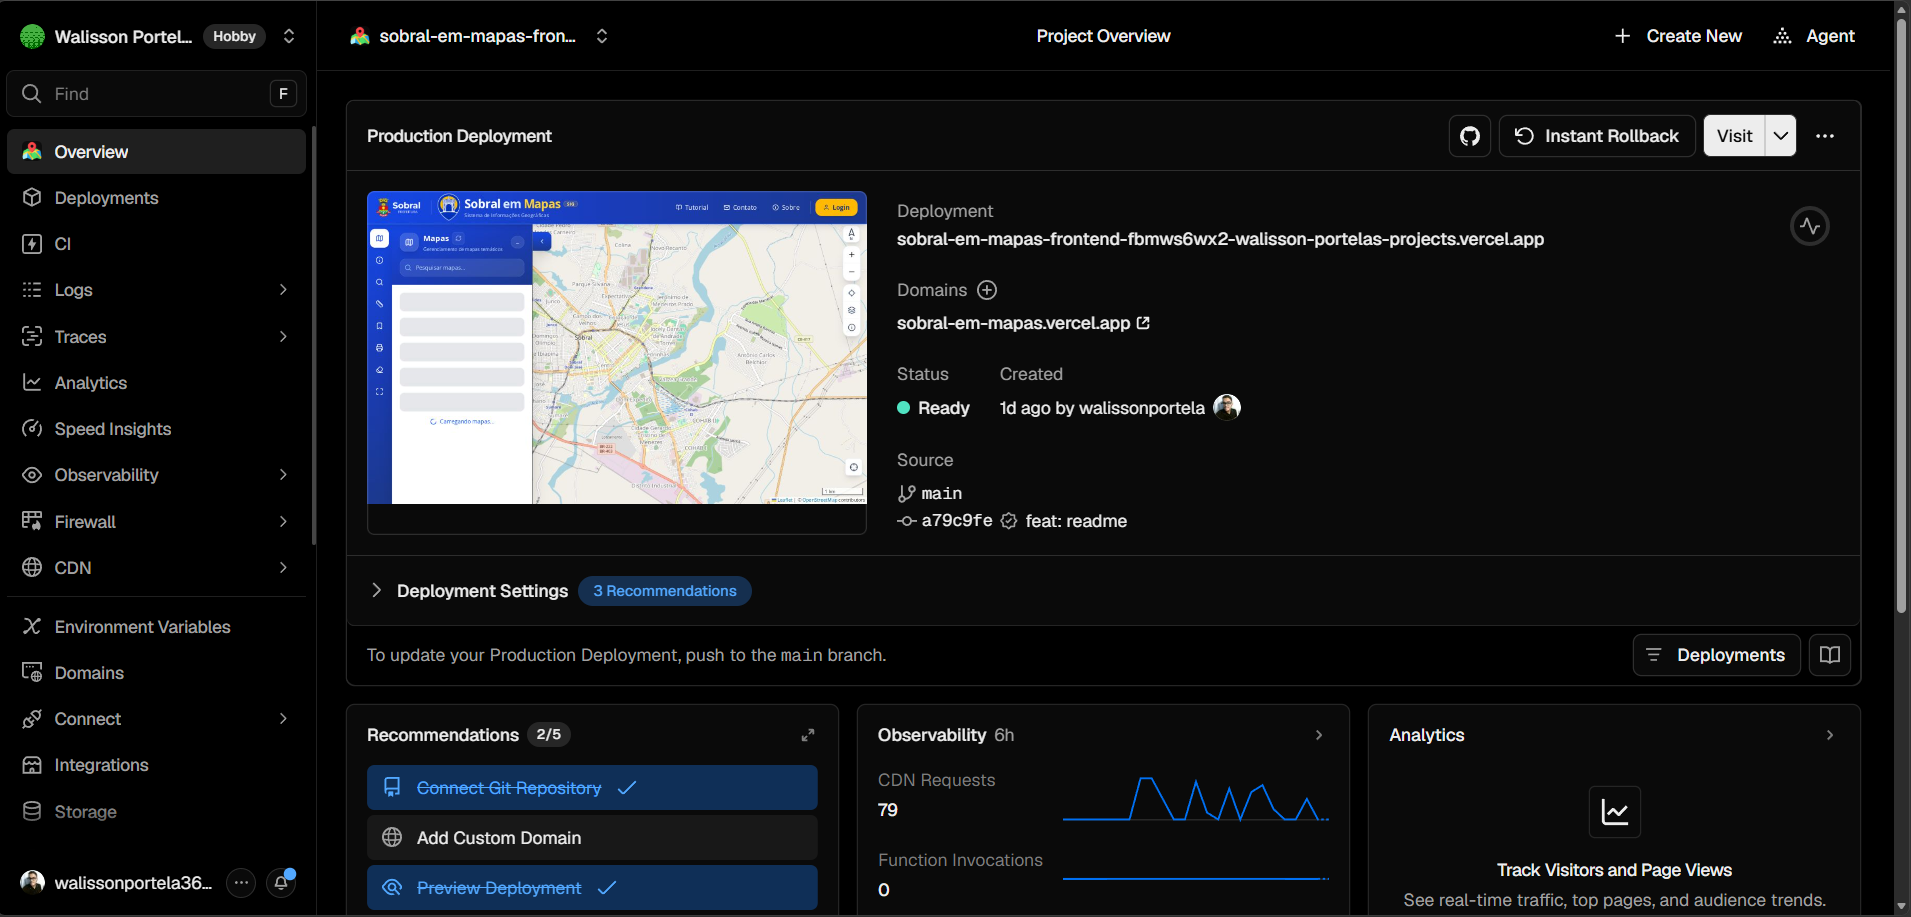
\includegraphics[width=1.0\textwidth,height=0.25\textheight,keepaspectratio]{figuras/implantacao-vercel.png}

    \par\smallskip

    {\footnotesize (a) Publicação do \textit{front-end} na Vercel}

    \par\medskip

    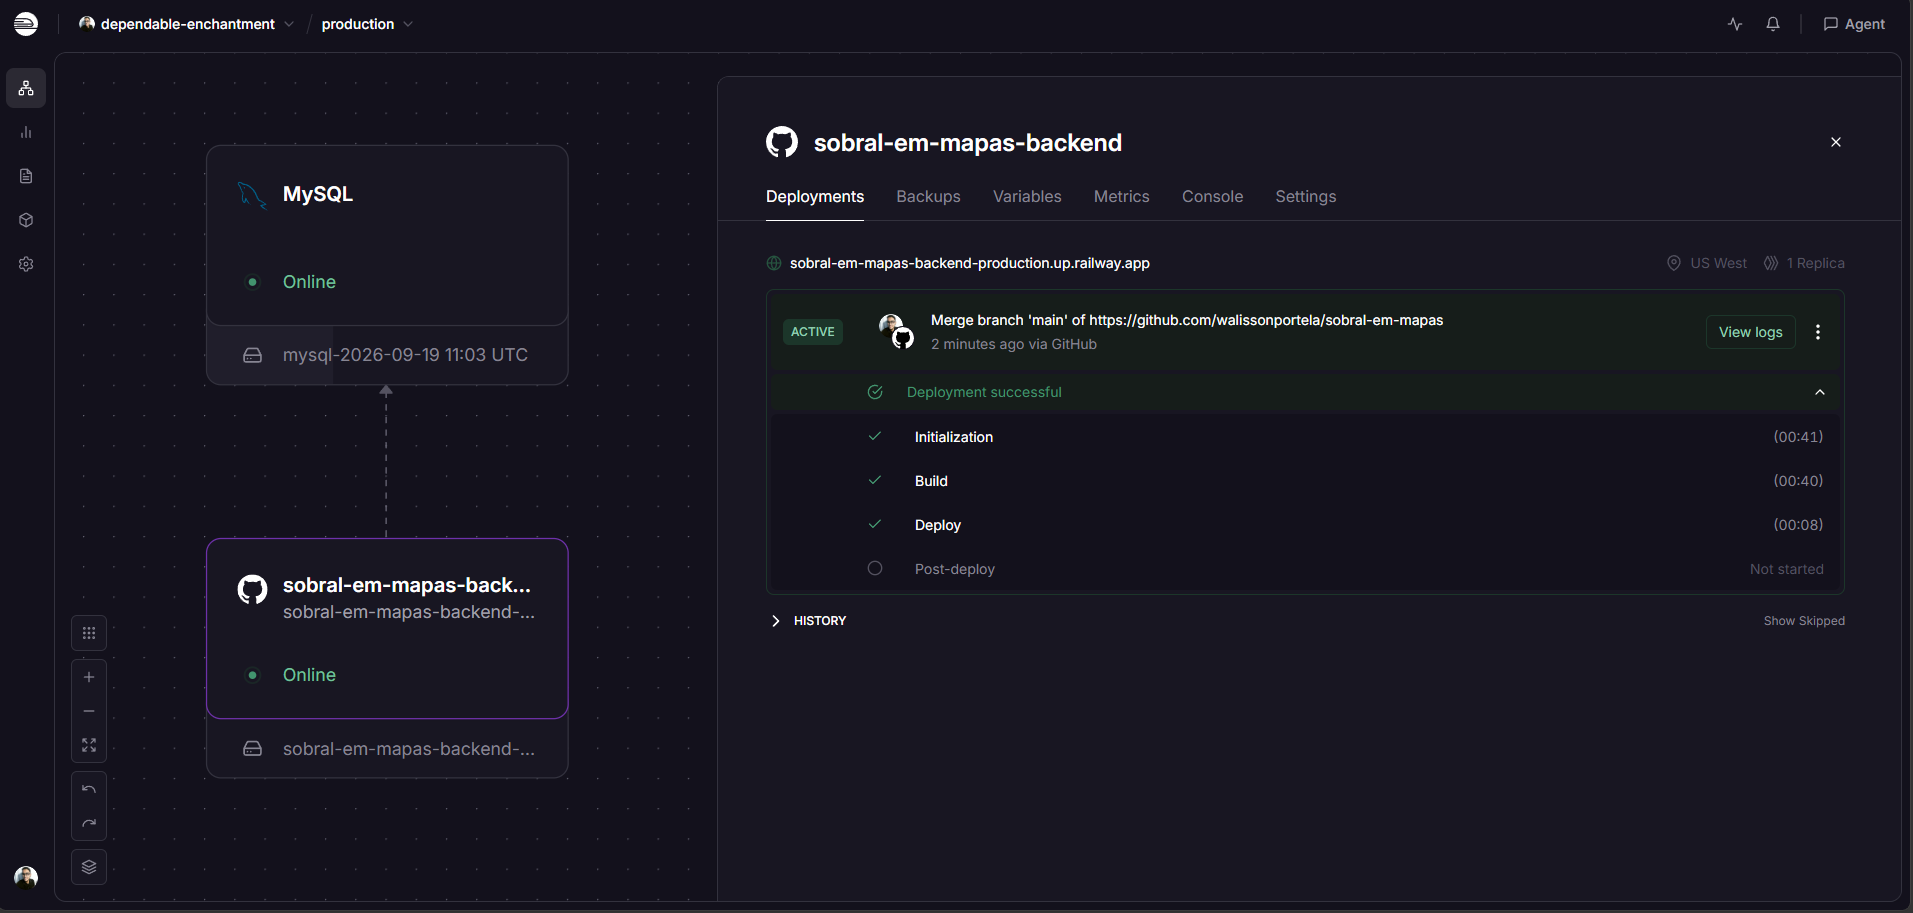
\includegraphics[width=1.0\textwidth,height=0.25\textheight,keepaspectratio]{figuras/implantacao-railway.png}

    \par\smallskip

    {\footnotesize (b) Execução da API no Railway}

    \par\medskip

    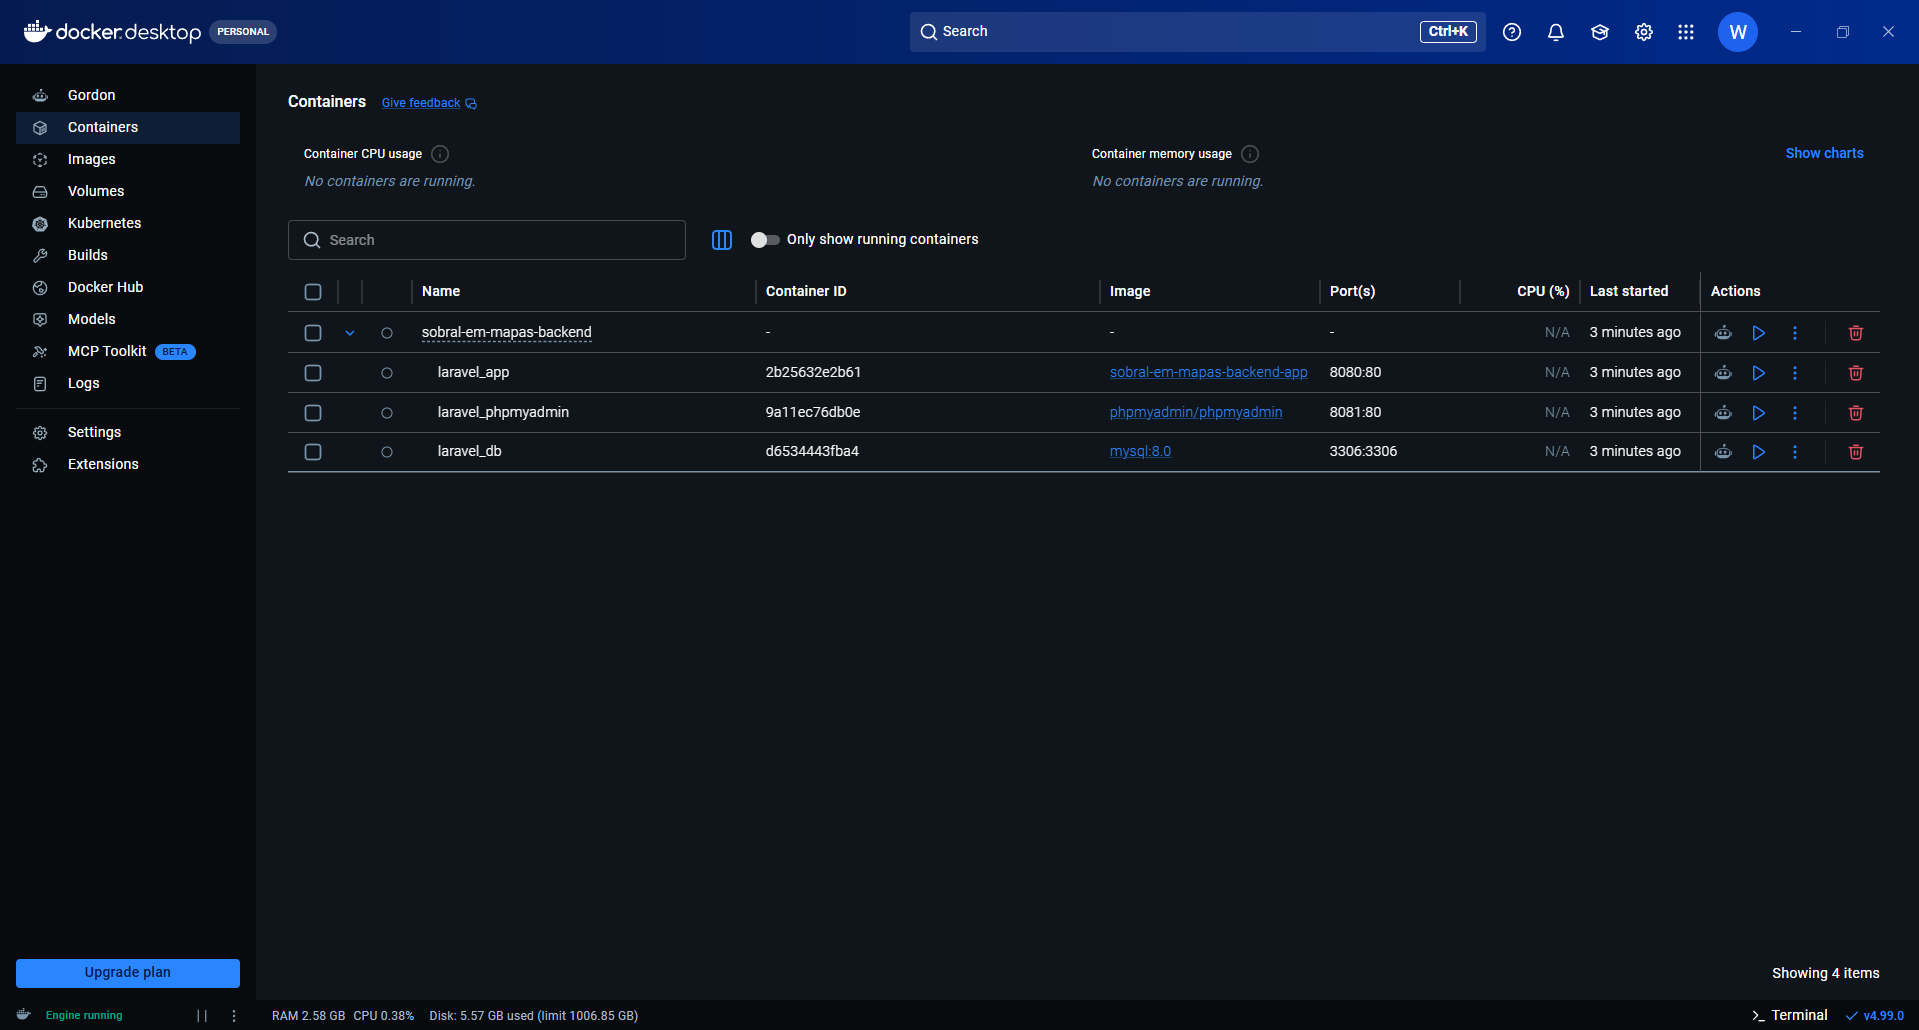
\includegraphics[width=1.20\textwidth,height=0.25\textheight,keepaspectratio]{figuras/implantacao-docker.png}

    \par\smallskip

    {\footnotesize (c) Ambiente local conteinerizado com Docker}

    \label{fig:implantacao-ambientes}

    \fonte{Capturas de tela realizadas pelo autor.}

\end{figure}

A utilização desses ambientes evidencia a separação entre a publicação da interface, a execução dos serviços administrativos e a preparação do ambiente local. Embora essa organização contribua para a disponibilização e a manutenção da plataforma, algumas limitações permanecem relacionadas à infraestrutura. Entre elas, destaca-se a dependência do GeoServer para o consumo dos serviços WMS, parcialmente contornada pela incorporação de arquivos GeoJSON como fonte adicional de dados geográficos. Além disso, a persistência desses arquivos exige configurações adequadas de armazenamento no ambiente de hospedagem.

\FloatBarrier

\section{Atendimento aos Requisitos}

\label{sec:atendimento-requisitos}

A análise do atendimento aos requisitos considerou as funcionalidades implementadas e os procedimentos de verificação descritos na Metodologia. Os resultados evidenciam a implementação dos principais recursos previstos, abrangendo a visualização cartográfica, as ferramentas de interação, o gerenciamento administrativo e a integração entre diferentes fontes geoespaciais. Para relacionar essas entregas ao planejamento do sistema, a Tabela~\ref{tab:atendimento-requisitos} apresenta os requisitos funcionais e seus respectivos recursos implementados.

\begin{table}[H]

    \captionsetup{width=15cm}

    \Caption{\label{tab:atendimento-requisitos} Relação entre requisitos funcionais e funcionalidades implementadas}

    \IBGEtab{}{

        \begin{tabular}{p{1.6cm}p{12.8cm}}

            \toprule

            \textbf{Código} &

            \textbf{Funcionalidade implementada} \\

            \midrule \midrule

            RF01 &

            Interface cartográfica interativa com camadas organizadas por categorias e subcategorias. \\

            \midrule

            RF02 &

            Pesquisa, ativação e desativação de camadas, com consulta às informações geográficas associadas. \\

            \midrule

            RF03 &

            Pesquisa de endereços e pontos de interesse, com localização dos resultados no mapa. \\

            \midrule

            RF04 &

            Ferramentas de medição de distâncias e áreas, além da criação, edição e armazenamento de geometrias GeoJSON no ambiente administrativo. \\

            \midrule

            RF05 &

            Recursos de favoritos, limpeza do mapa, tela cheia e impressão ou exportação cartográfica. \\

            \midrule

            RF06 &

            Formulário de contato integrado à API para encaminhamento de mensagens. \\

            \midrule

            RF07 &

            Cadastro, autenticação e controle de acesso conforme os perfis e a situação de aprovação dos usuários. \\

            \midrule

            RF08 &

            Gerenciamento administrativo de usuários, perfis de acesso e solicitações de aprovação. \\

            \midrule

            RF09 &

            Cadastro e manutenção de categorias e subcategorias utilizadas na organização das camadas. \\

            \midrule

            RF10 &

            Gerenciamento de camadas WMS e GeoJSON, incluindo metadados, envio de arquivos e pré-visualização cartográfica. \\

            \bottomrule

        \end{tabular}

    }{

        \Fonte{Elaborado pelo autor.}

    }

\end{table}

Os requisitos não funcionais contemplam responsividade, separação de responsabilidades, integração com WMS e GeoJSON, autenticação, autorização e validação de dados. Também foram utilizados componentes React reutilizáveis, comunicação HTTP/HTTPS, Docker e variáveis de ambiente. Essas decisões atendem a aspectos técnicos previstos, embora segurança, desempenho e responsividade ainda exijam testes em diferentes condições.

De modo geral, foram implementadas as principais funcionalidades previstas. O suporte a arquivos GeoJSON permite disponibilizar camadas sem depender apenas dos serviços WMS externos, reduzindo os efeitos das limitações dessa infraestrutura.

\section{Avaliação com Usuários}

\label{sec:avaliacao-usuarios}

Para complementar as verificações funcionais, foi iniciada uma avaliação exploratória de usabilidade, na qual participantes convidados executam atividades na interface pública e no ambiente administrativo do ``Sobral em Mapas''. Após a consulta às camadas, a utilização das ferramentas cartográficas e as operações de gerenciamento orientadas por um guia de teste, os participantes foram convidados a responder voluntariamente a um questionário eletrônico sobre facilidade de uso, compreensão das informações e experiência geral.

\section{Discussão dos Resultados e Limitações}

\label{sec:discussao-resultados}

Os resultados apresentados demonstram a implementação de uma plataforma WebGIS que reúne recursos de consulta, visualização e gerenciamento de informações geoespaciais do município de Sobral. A organização temática das camadas, as ferramentas cartográficas e o ambiente administrativo evidenciam a integração entre os componentes desenvolvidos. Além disso, a separação entre \textit{front-end}, \textit{back-end} e fontes de dados contribuiu para estruturar a solução e incorporar novas funcionalidades ao longo do desenvolvimento.

Entre os resultados obtidos, destaca-se a ampliação do suporte a dados geoespaciais por meio do formato GeoJSON, que permite incorporar arquivos vetoriais, consultar atributos e criar ou editar geometrias no ambiente administrativo. Dessa forma, a plataforma passou a oferecer uma alternativa complementar aos serviços WMS, reduzindo a dependência exclusiva de infraestrutura externa para disponibilizar camadas cartográficas.

Entretanto, algumas limitações permanecem associadas à arquitetura adotada, visto que o consumo de camadas WMS depende da disponibilidade dos serviços fornecidos pelo GeoServer, enquanto os arquivos GeoJSON exigem armazenamento e persistência adequados no servidor de aplicação. Ademais, o processamento de conjuntos geográficos extensos diretamente no navegador pode afetar o desempenho, sobretudo em dispositivos com recursos computacionais limitados, aspecto que ainda demanda verificações específicas.

Embora as funcionalidades implementadas indiquem a viabilidade técnica da solução, são necessárias avaliações com diferentes perfis de usuários. As verificações funcionais oferecem evidências do comportamento dos recursos, enquanto a avaliação com usuários, ainda em coleta, deverá identificar percepções de usabilidade e dificuldades de interação.